\scanpage{115}
\mspage{705}

\[
\tag{267}
\left\{
\begin{gathered}
\unsure{\rho'}=\zeta\rho,\ \sigma'=\eta\sigma
\quad(\zeta,\eta\in\Gamma\underline M)\quad\text{such that we have}
\\
\rho'{}^3=\sigma'{}^2=\omega,\qquad
\sigma'(\rho')=\rho'{}^{-1}.
\end{gathered}\right.
\]

(We \unsure{note|shall note} that a splitting must transform $\omega$,
which operates trivially on $\underline M$ and is central
in $\underline H^+$, into a central \deleted{\unsure{element}}
\inserted{section}, \unsure{now}
\deleted{\unsure{the inverse}} \unsure{see|here is} \unsure{why} we have
\[
\tag{268}
\left\{\begin{aligned}
\underline M\cap\underline{\mathrm{Cent}}\bigl(\underline{\mathfrak S}^+\bigr)
&=\underline M^{\mathfrak S_3}
=\deleted{\unsure{\{0\}}}\,\unsure{\{1\}|\{0\}},\quad\text{hence}
\\
\underline{\mathrm{Cent}}\bigl(\underline{\mathfrak S}^+\bigr)
&\simeq\underline\mu_{\underline{\mathfrak S}}
=\{1,\omega\}_{\underline{\mathfrak S}}
\end{aligned}\right.
\]
--- which shows that a splitting must transform $\omega$ into $\omega$,
whence \unsure{easily} the characterization (267) of the $\rho',\sigma'$
\unsure{corresponding|corresponding} to a splitting).
We shall have from this
\[
\left\{\begin{aligned}
\rho'{}^3&=(\zeta\rho)^3
=\zeta\rho(\zeta)\rho^2(\zeta)\underbrace{\rho^3}_{\omega}
=\zeta\rho(\zeta)\rho^2(\zeta)\omega
\\
\sigma'{}^2&=(\eta\sigma)^2
=\eta\sigma(\eta)\underbrace{\sigma^2}_{\omega}
=\eta\sigma(\eta)\omega
\end{aligned}\right.
\]
thus the \deleted{two} equations $\rho'{}^3=\omega$ and
$\sigma'{}^2=\omega$ are equivalent respectively to
\[
\left\{\begin{aligned}
\zeta\rho(\zeta)\rho^2(\zeta)&=1
&\text{i.e.}\quad(1+\rho_M+\rho_M^2)(\zeta)&=0
\\
\eta\sigma(\eta)&=1
&\text{i.e.}\quad(1+\sigma_M)(\eta)&=0
\end{aligned}\right.
\]
i.e. this reduces to equations (245) (246),
and we have seen that the \deleted{general solution is}
\inserted{\deleted{first} condition}
on $\zeta$ is automatically satisfied, that
on $\eta$ amounts to:
\[
(247)\qquad
\eta=b\delta=b(\lambda_1-\lambda_0),\quad
\unsure{\lambda|b}\in\Gamma\mathbb G_a.
\]
The condition $\sigma'(\rho')=\rho'{}^{-1}$ is made explicit on the other
hand as on page~$700'$, we come back

\margin{114}

\begin{center}
\small
114\\
\texttt{https://grothendieck.umontpellier.fr}\\
Université de Montpellier, UMR CNRS 5149, Case courrier 051, Place Eugène Bataillon\\
34095 Montpellier cedex 5 - France
\end{center}

\scanpage{116}

to equation (249), which is made explicit by (250).
This shows that there exists a splitting
even over $S_0=\mathrm{Spec}\,\mathbb Z$
--- which amounts to a splitting \unsure{of the} discrete group
$\mathfrak S^+$ extension of
$H^+=\mathfrak S^+/M$
\inserted{$\simeq\mathfrak S_0/\Pi_0$}
(by $M\simeq(\Pi_0)_{\mathrm{ab}}$ \unsure{)}
--- and that the splittings in question form a
torsor under $\underline K$, where $K$\inserted{$\simeq\mathbb Z^2$}
is defined in (253), and in fact \deleted{\unsure{$K$}}
we have an isomorphism $M\simeq K$ (254), i.e.
$\underline M\simeq\underline K$, \unsure{corresponding}
to the operation of $\underline M$ on the \unsure{scheme}
of splittings, by conjugation. Thus we find

\uline{Proposition} (Over an arbitrary base $S$).

The extension $\underline{\mathfrak S}^+$ of
$\underline H^+$ by $\underline M$ is split ---
two splittings are conjugate by a unique section
of $\underline M$ --- thus the map \deleted{of}
``passage to the quotient by $\mu_{\mathfrak S}$'' defines a
bijection from the \unsure{set} of splittings of
$\underline{\mathfrak S}^+$ over $\underline H^+$,
onto the \unsure{set} of splittings of
$\underline{\mathfrak S}^+/\mu_{\underline{\mathfrak S}}$
over $\underline H^+/\underline\mu_{\underline H^+}
\simeq\underline{\mathfrak S}_3$.

\margin{115}

\begin{center}
\small
115\\
\texttt{https://grothendieck.umontpellier.fr}\\
Université de Montpellier, UMR CNRS 5149, Case courrier 051, Place Eugène Bataillon\\
34095 Montpellier cedex 5 - France
\end{center}

\scanpage{117}
\mspage{706}

Let us now study the centralizer in
$\underline G_{\rho,\sigma}$ of a section subgroup
over $\underline H^+$, \unsure{say} denoted
$\underline H(\rho',\sigma')$. We must now have
\[
\tag{269}
\underline{\mathrm{Cent}}_{\underline G_{\rho,\sigma}}
\bigl(\underline H(\rho',\sigma')\bigr)
\subset
\begin{gathered}
\mathbb O_{12}^*\cdot\bigl(\underline M\times
\underbrace{\mu_{\underline{\mathfrak S}}}_{=\{1,\omega\}_{S_0}}\bigr)
\\[-2pt]
\Vert
\\[-2pt]
\left\{\lambda\omega^i u_{\underline\mu}\ \middle|\
\begin{gathered}
\lambda\in\Gamma\underline M\\
\underline\mu\in\Gamma\mathbb O_{12}^*\\
i\in\Gamma(\unsure{\mathbb Z/2\mathbb Z})_{S_0}
\end{gathered}\right\}
\end{gathered}
\]
Moreover $\lambda\omega^i u_{\underline\mu}$ centralizes
$\underline H(\rho',\sigma')$ iff $\lambda u_{\underline\mu}$
centralizes. Commutation with $\rho'$ is again made explicit
by condition (260), the calculation on page~703 applying
\unsure{ne varietur}. For the condition of commutation with
$\sigma'$, the calculation on page~$703'$ must be modified
for we can no longer write $\omega^{\nu_2}=1$,
the condition is written
\[
\omega^{\nu_2}\cdot\lambda\eta^{\unsure{\mu}}
\sigma(\lambda^{-1})\sigma=\eta\sigma
\quad\text{i.e.}\quad
\omega^{\nu_2}\lambda\eta^\mu\sigma(\lambda^{-1})=\eta
\]
and is equivalent to the conjunction of the condition
\[
\tag{270}
\nu_2(\underline\mu)=0\quad\text{i.e.}\quad
\underline\mu\in\Gamma\mathbb O_{12}^{*\prime\prime},
\]
and of relation (261). In the presence of
$\nu_2(\underline\mu)=0$, the calculations on pages~$703'$, 704
apply, \unsure{finally} we find:

\uline{Corollary} For every splitting of
$\underline{\mathfrak S}^+$ over
$\underline H^+$, \deleted{the commutant}
\inserted{\deleted{\illegible{1}} let $\underline T$ be the centralizer
\deleted{\unsure{$T$}}} in $\underline G_{\rho,\sigma}$
of the section subgroup $\underline H(\rho',\sigma')$,
\deleted{we}

\margin{116}

\begin{center}
\small
116\\
\texttt{https://grothendieck.umontpellier.fr}\\
Université de Montpellier, UMR CNRS 5149, Case courrier 051, Place Eugène Bataillon\\
34095 Montpellier cedex 5 - France
\end{center}

\scanpage{118}

\deleted{\unsure{a section}}\inserted{We then have} an exact sequence
\[
\tag{271}
\diagram{\begin{tikzcd}[column sep=large]
1 \arrow[r] & \underline\mu_{\unsure{\mathfrak S|G}}
\arrow[r,hook,"{\deleted{\unsure{G}}}" description]
& \underline T \arrow[r] & \mathbb O_{12}^{*\prime\prime}
\arrow[r,no head] & 1
\end{tikzcd}}
\]
and for $\underline T^{\unsure{\natural|\sharp}}
=\underline T\cap\underline G_{\rho,\sigma}^{\unsure{\natural|\sharp}}$,
we have
\[
\tag{272}
\underline T^{\unsure{\natural|\sharp}}
\simeq\mathbb O_{12}^{*\prime\prime},
\]
i.e. $\underline T^{\unsure{\natural|\sharp}}$ is a partial
section of $\underline G_{\rho,\sigma}^{\unsure{\natural|\sharp}}$
over $\mathbb O_{12}^{*\prime\prime}$.

\uline{Corollary} The extension $\underline G_{\rho,\sigma}$ of
$\mathbb O_{12}^*\times\underline H^+$ by $\underline M$
is not split over any nonempty base $S$.
The extension $\underline G_{\rho,\sigma}''$ of
$\mathbb O_{12}^{*\prime\prime}\times\underline H^+$ by
$\underline M$ is split over every base $S$,
and two splittings are conjugate by a unique section of
$\underline M$. The natural map gives a bijection
of the \unsure{set} of splittings of $\underline G_{\rho,\sigma}''$
over $\mathbb O_{12}^{*\prime\prime}\times\underline H^+$, with
the \unsure{set} of splittings of
$\underline{\mathfrak S}^+$ over $\underline H^+$.

\uline{Corollary} The extension $G_{\rho,\sigma}$ of
$\widehat{\mathbb Z}^{*}\times H^+$ by $M^\wedge$
is not split. That of $G_{\rho,\sigma}''$ of
$\widehat{\mathbb Z}^{*\prime\prime}\times H^+$ by
$M^\wedge$ is split, and two splittings are
conjugate by a unique element \unsure{of} $\widehat M$.
The natural map defines a bijection of the \unsure{set}
of splittings of $G_{\rho,\sigma}''$ over
$\widehat{\mathbb Z}^{*}\times H^+$ with the \unsure{set}
of splittings of \deleted{\unsure{$G_\rho$}}
$\mathfrak S^\wedge$ over $H^+$.

\margin{117}

\begin{center}
\small
117\\
\texttt{https://grothendieck.umontpellier.fr}\\
Université de Montpellier, UMR CNRS 5149, Case courrier 051, Place Eugène Bataillon\\
34095 Montpellier cedex 5 - France
\end{center}

\scanpage{119}
\mspage{707}

Let us make explicit a splitting of the extension
$\mathfrak S^+$ of $H^+$ by $M$
--- corresponding to a splitting of
$\underline{\mathfrak S}^+$ of $\underline H^+$
by $\underline M$ --- , via a particular solution of the equation
\[
\tag{273}
a_0-2a_1+3b-1=0
\]
taking
\[
a_1=b=0\qquad\text{hence}\qquad a_0=1
\]
i.e.
\[
\tag{274}
\left\{\begin{aligned}
\zeta&=\lambda_0,\ \eta=0\quad\text{(additive notation)}\\
\rho'&=\lambda_0\rho,\quad\unsure{\sigma'}=\unsure{\sigma}
\end{aligned}\right.
\]
\deleted{the corresponding splitting}
\inserted{the \unsure{three} formulas give a splitting of
$\mathfrak S^+/\mu_{\mathfrak S}$}
over $\mathfrak S_3
\simeq H^+/\mu_{H^+}$.
Let us make explicit the \unsure{corresponding}
\deleted{splittings}\inserted{liftings} of $\mathbb O_{12}^*$ into
$\underline G_{\rho,\sigma}/\mu_G$ resp. of
$\mathbb O_{12}^{*\prime\prime}$ into $\underline G_{\rho,\sigma}$\unsure{;},
\[
\tag{275}
\left\{\begin{aligned}
u_{\rho',\sigma'}:\mathbb O_{12}^*&\longrightarrow
\underline G_{\rho,\sigma}/\mu_G
\quad\text{resp.}\quad\mathbb O_{12}^{*\prime\prime}
\mathrel{\text{---}}\underline G_{\rho,\sigma}
\\
\underline\mu&\longmapsto\lambda_\infty^{\nu}u_{\underline\mu}
\qquad(\nu=\nu(\underline\mu))
\end{aligned}\right.
\]
where $u_{\underline\mu}$ defined in (151).
(N.B.\unsure{\S} (275) is contained in proposition page~704
(265) and (264), which give
\[
u_{\rho',\sigma'}=\lambda u_{\underline\mu}\qquad
\lambda=x\lambda_0+y\lambda_1\qquad x=y=-\nu
\]
\[
\text{hence}\qquad\lambda=-\nu(\lambda_0+\lambda_1)=\nu\lambda_\infty.
\]

We shall thus have, putting
\[
u'_{\underline\mu}=u_{\rho',\sigma'}(\underline\mu)
\]
\[
\tag{276}
\left\{\begin{aligned}
u'_{\underline\mu}(\rho')&=\rho',\quad
u'_{\underline\mu}(\sigma')=\sigma'\\
u'_{\underline\mu}(\lambda)&=\mu\lambda\quad
(\lambda\in\Gamma\underline M)
\quad\inserted{\text{where}}\ (\mu=\unsure{\chi}(\underline\mu))
\end{aligned}\right\}
\quad\begin{gathered}
\text{(which suffices}\\
\text{to \unsure{condition|characterize}}\ u'_{\underline\mu})
\end{gathered}
\]

\margin{118}

\begin{center}
\small
118\\
\texttt{https://grothendieck.umontpellier.fr}\\
Université de Montpellier, UMR CNRS 5149, Case courrier 051, Place Eugène Bataillon\\
34095 Montpellier cedex 5 - France
\end{center}

\scanpage{120}

and we also deduce from this
\[
\tag{277}
\left\{
\begin{aligned}
u'_{\underline{\mu}}(\rho)&=\lambda_0^{-2\nu}\rho\\
u'_{\unsure{\mu|\underline{\mu}}}(\sigma)&=\omega^{\nu_2}\sigma
\qquad (=\sigma\text{ in }\underline G_{\rho,\sigma}/\underline{\mu}_G\ \ldots).
\end{aligned}
\right.
\]

\margin{119}

\begin{center}
\small
119\\
\texttt{https://grothendieck.umontpellier.fr}\\
Université de Montpellier, UMR CNRS 5149, Case courrier 051, Place Eugène Bataillon\\
34095 Montpellier cedex 5 - France
\end{center}

\scanpage{121}
\mspage{708}

13\textsuperscript{o}) \uline{Return to the Fermat tower}.

Let us begin by bringing out a general topossic notion, which \unsure{was} a little
muddled between the lines in 11\textsuperscript{o}).
Let $\Gamma$ (here $\Gamma_{\mathbb Q}\times
\mathfrak S_3\deleted{\unsure{)|\}}}=N_{0,3}$) be operating on
a topos $\mathcal X$ (here
$\deleted{\unsure{U}}\inserted{\unsure{\mathcal U}_{0,3\overline{\mathbb Q}}}
\simeq M'_{0,4\overline{\mathbb Q}}$) connected
\inserted{locally connected}, \deleted{\unsure{and connected}} equipped with a ``point'' (geometric)
$x_0$ (here: the point $-\overline j$ with values in $\overline{\mathbb Q}$), let
\margin{Discrete context ($\mathcal X$ locally simply connected) or profinite,
\unsure{relatively}\illegible{1} \unsure{reasonable}\ldots}
\[
\tag{278}
\left\{
\begin{aligned}
\Pi&=\Pi_1(\mathcal X,x_0),\qquad
\mathcal M=\Pi_1(\mathcal X,\Gamma;x_0)\\
M&=\Pi_{\mathrm{ab}}=\Pi/[\Pi,\Pi],\qquad
\deleted{\unsure{\mathfrak S}}\inserted{\widetilde{\mathcal M}}
=\mathcal M/[\Pi,\Pi],\qquad \deleted{\text{hence}}
\end{aligned}
\right.
\]
hence exact sequences and homomorphisms of exact sequences
\[
\tag{279}
\diagram{\begin{tikzcd}[column sep=large,row sep=large]
1 \arrow[r,dash] & \Pi \arrow[r] \arrow[d,"\text{epimorphism}"]
& \mathcal M \arrow[r] \arrow[d,"\text{epimorphism}"]
& \Gamma \arrow[r,dash] \arrow[d,"\unsure{\sim|\wr}"] & 1\\
1 \arrow[r,dash] & M \arrow[r,dash]
& \deleted{\unsure{\mathfrak S}}\inserted{\widetilde{\mathcal M}} \arrow[r]
& \Gamma \arrow[r,dash] & 1
\end{tikzcd}}\ .
\]

\deleted{Let us consider}
\inserted{(Instead of taking
$M=\Pi/\unsure{(\Pi,\Pi)|[\Pi,\Pi]}\inserted{=\Pi_{\mathrm{ab}}}$,}
we \unsure{would have|had} been able to take a quotient of $\Pi_{\mathrm{ab}}$ invariant under
the action of $\Gamma$, but no matter\ldots).
Let us consider ``the universal abelian covering'' \inserted{$\mathcal X'_0$} of
$\mathcal X$ at $x_0$, i.e. the quotient by $[\Pi,\Pi]$ of the universal covering of
$\mathcal X$ at $x_0$ --- it is thus a principal covering of $\mathcal X$, with
group $M$. We

\margin{120}

\begin{center}
\small
120\\
\texttt{https://grothendieck.umontpellier.fr}\\
Université de Montpellier, UMR CNRS 5149, Case courrier 051, Place Eugène Bataillon\\
34095 Montpellier cedex 5 - France
\end{center}

\scanpage{122}

proposes to examine the ways of \deleted{extending}\inserted{lifting}
the action of $\Gamma$ on $\mathcal X$ \deleted{(via $M$)} to an
action \deleted{of $\mathcal M$}\inserted{on $\mathcal X'_0$}, compatible
with the action \inserted{of $\Gamma$ on the group of operators $M$}
\deleted{on $\mathcal X$ via $\Gamma$,
\inserted{and extend the action of
$M\subset\mathfrak S$,}
\unsure{or what} \unsure{amounts} to the same thing, by an action of
$\mathfrak S$, compatible with its action on
$\mathcal X$ (via $\Gamma$)}.
More generally, if $\mathcal X'$ is an $M_{\mathcal X}$-torsor on
$\mathcal X$ isomorphic \unsure{to} $\mathcal X'_0$, hence obtained
\deleted{\unsure{by a}}\inserted{from $\mathcal X'_0$} by twisting with
an $M$-torsor $E$ ($\unsure{\simeq|=}$ fiber of $\mathcal X'_0$ at $x_0$),
let us study the analogous \deleted{extensions}\inserted{liftings} of the action
of $\deleted{\unsure{\mathfrak S}}\inserted{\Gamma}$ on $\mathcal X$ to an
action of $\deleted{\unsure{\mathfrak S}}\inserted{\Gamma\text{ on }\mathcal X'}$,
compatible with the action of
$\deleted{\unsure{\mathfrak S}}\inserted{\Gamma}$ on $\mathcal X$.

\deleted{Note that, if $\widetilde{\mathcal X}$ denotes the universal covering of
$\mathcal X$ at $x_0$, $\mathcal M$ operates on $\widetilde{\mathcal X}$ in a way
compatible with its action on $\mathcal X$, \unsure{while|and} extending the
\inserted{canonical} action of $\Pi$ on $\widetilde{\mathcal X}$ --- as
$[\Pi,\Pi]\subset\Pi$ is normal in $\mathcal M$, this action passes to the
quotient as a canonical action of
$\mathfrak S=\mathcal M/[\Pi,\Pi]$ on
$\mathcal X'_0=\widetilde{\mathcal X}/[\Pi,\Pi]$, which satisfies the}

\margin{121}

\begin{center}
\small
121\\
\texttt{https://grothendieck.umontpellier.fr}\\
Université de Montpellier, UMR CNRS 5149, Case courrier 051, Place Eugène Bataillon\\
34095 Montpellier cedex 5 - France
\end{center}

\scanpage{123}
\mspage{709}

\deleted{\inserted{two} conditions envisaged. Let $\Theta_0$ be this
operation of $\mathfrak S$, and $\Theta$ an arbitrary operation,
satisfying the said conditions.}

We thus want to make $\mathcal X'$, which is a covering of $\mathcal X$, given
by its fiber $E$ at $x_0$ and the action of $\Pi=\Pi_1(\mathcal X,x_0)$ on
$E$ (by translations, thanks to an $M$ torsor structure on $E$) into a
covering of $(\mathcal X',\deleted{\unsure{\mathfrak S}}\inserted{\Gamma})$
--- i.e. \uline{extend} the given action of $\Pi$ on \unsure{the|the} fiber
$E$, to an action of $\mathcal M$ on $E$ --- which moreover necessarily factors
through
$\deleted{\unsure{\mathfrak S}}\inserted{\widetilde{\mathcal M}}$.
I say that this action necessaril\textsuperscript{y} goes \unsure{by} way of the
affine group of the torsor $E$ --- to be precise, $\Gamma$ operates on $M$,
\unsure{let} $\gamma_M$ be the operation defined by $\gamma\in\Gamma$, and let
$g\in\deleted{\unsure{\mathfrak S}}\inserted{\widetilde{\mathcal M}}$ be over
$\gamma\in\Gamma$, we will thus have, for $x\in E$, $\lambda\in M$
\[
\tag{280}
\diagram{\begin{tikzcd}[column sep=0em,row sep=0.6em]
g & (\lambda & {}\cdot{} & x & {})=\gamma_M(\lambda)\mathbin{.}gx\\
\deleted{\unsure{\mathfrak S}}\inserted{\widetilde{\mathcal M}}
\arrow[u,phantom,"\in"{description,rotate=-90}]
& M\arrow[u,phantom,"\in"{description,rotate=-90}]
& & E\arrow[u,phantom,"\in"{description,rotate=-90}] &
\end{tikzcd}}
\]
which \unsure{is} trivial by calculation.
\deleted{\unsure{for|is}}
\[
g(\lambda.x)=(g\lambda)x=(g\lambda g^{-1}g)x
=\underbrace{(g\lambda g^{-1})}_{\gamma_M(\lambda)}.(gx)
\]

\margin{122}

\begin{center}
\small
122\\
\texttt{https://grothendieck.umontpellier.fr}\\
Université de Montpellier, UMR CNRS 5149, Case courrier 051, Place Eugène Bataillon\\
34095 Montpellier cedex 5 - France
\end{center}

\scanpage{124}

Thus if we introduce the group $\operatorname{Aff}(E)$, we will have a
homomorphism of exact sequences
\[
\tag{281}
\diagram{\begin{tikzcd}[column sep=large,row sep=large]
1 \arrow[r] & M \arrow[r,dash]
\arrow[d,Rightarrow,"{\deleted{\unsure{\Theta}}\mathrm{id}_M}"]
& \deleted{\unsure{\mathfrak S}}
\inserted{\widetilde{\mathcal M}} \arrow[r]
\arrow[d,"{\Theta_{\deleted{\unsure{\mathfrak S}}\inserted{\widetilde{\mathcal M}}}}"]
& \Gamma \arrow[r,dash] \arrow[d,"\Theta_\Gamma"] & 1\\
1 \arrow[r,dash] & M \arrow[r]
& \operatorname{Aff}(E) \arrow[r]
& \operatorname{Aut}(M) \arrow[r] & 1
\end{tikzcd}}
\]
where the outer vertical arrows $\mathrm{id}_M$ \inserted{and
$\Theta_\Gamma$} are known, and where the middle arrow is to be determined.
We can say that the category of the $\mathcal X'$ \unsure{sought|sought}
(with the operation of $\Gamma$ on them satisfying the desired conditions)
\inserted{is} equivalent to that of pairs
$(E,\Theta_{\deleted{\unsure{\mathfrak S}}\inserted{\widetilde{\mathcal M}}})$,
where $E$ is an $M$-torsor, and
$\Theta_{\deleted{\unsure{\mathfrak S}}\inserted{\widetilde{\mathcal M}}}$
a homomorphism of groups
$\deleted{\unsure{\mathfrak S}}\inserted{\widetilde{\mathcal M}}
\longrightarrow\operatorname{Aff}(E)$ \deleted{\unsure{making}}
compatible with $\mathrm{id}_M$ and $\Theta_\Gamma$ i.e. which
\unsure{makes|makes} (281) commutative.
We can also say: once $E$ is chosen,
\inserted{(and this choice is \unsure{harmless} up to nonunique
isomorphism\unsure{!!!|\ldots})}
that this defines an extension $\operatorname{Aff}(E)$ of
$\operatorname{Aut}(M)$ by $M$, whence thanks to
$\Gamma\longrightarrow\operatorname{Aut}(M)$ an
extension

\margin{123}

\begin{center}
\small
123\\
\texttt{https://grothendieck.umontpellier.fr}\\
Université de Montpellier, UMR CNRS 5149, Case courrier 051, Place Eugène Bataillon\\
34095 Montpellier cedex 5 - France
\end{center}

\scanpage{125}
\mspage{\textcircled{710}}

\margin{the splittings of $\operatorname{Aff}(E)$ determined by the points of $E$ -- \unsure{shift} of the origin \unsure{inner} \unsure{splittings}\ldots}

by $M$, \inserted{which is \uline{moreover split}.} (That said, the liftings of the action of $\Gamma$ on it correspond to the isomorphisms of this extension of $\Gamma$ by $M$, with the extension $\mathfrak S$ itself. Thus it exists iff the extension of $\mathfrak S$ of $\Gamma$ by $M$ is split, \deleted{\unsure{which}} \inserted{i.e.\ \unsure{the expression}}
\[
c^2(\mathfrak S)\in H^2(\Gamma,M)\quad\text{is zero.}
\tag{282}
\]
If such a lifting exists i.e. such an isomorphism, these form a torsor \unsure{under|over} the group of automorphisms of the extension (trivial) $\mathfrak S$ of $\Gamma$ by $M$ which is identified with the group
\[
(\qquad Z^1(\Gamma,M)
\]
of crossed homomorphisms from $\Gamma$ to $M$. The $M$-conjugacy classes of such \deleted{liftings \unsure{(or}} isomorphisms therefore correspond to the elements of
\[
H^1(\Gamma,M).
\]

Another way of saying it, by taking $E={}$trivial \inserted{$M$-}torsor${}=M$, so $\operatorname{Aff}(E)$ split, is that the chosen liftings correspond to the \uline{splittings} of the extension $\mathfrak S$ of $\Gamma$ by $M$, and the \inserted{$M$-}conjugacy classes of the liftings of the action of $\Gamma$ on $\mathcal X'_0$

\margin{124}

\begin{center}
\small
124\\
\texttt{https://grothendieck.umontpellier.fr}\\
Université de Montpellier, UMR CNRS 5149, Case courrier 051, Place Eugène Bataillon\\
34095 Montpellier cedex 5 - France
\end{center}

\scanpage{126}

correspond to the $M$-conjugacy classes of the splittings of the said extension $\mathfrak S$ of $\Gamma$ by $M$.

This being well set out, let us return to the situation of
\[
\left(\underbrace{U_{0,3\overline{\mathbb Q}}}_{\mathcal X},\quad
\Gamma=\underbrace{\Gamma_{\mathbb Q}\times\mathfrak S_3}_{N_{0,3}}\right),
\]
the $\Gamma$-coverings of $\mathcal X$ correspond to the $\mathfrak S_3$-coverings of $U_{0,3\mathbb Q}$, i.e. to the coverings of $(U_{0,3\mathbb Q},\mathfrak S_3)$.

\margin{\uline{N.B.} The group we have just denoted $M$ becomes here $\unsure{\widehat M}$, $\mathcal M$ becomes $\mathcal M_{0,3}$, $\pi$ becomes $\widehat\Pi_{0,3}$.}

Using the general constructions of \S~49 $\overline{\uline{\mathrm{VI}}}$, \deleted{we deduced} from the quotient
\[
\deleted{\unsure{G_{\rho,\sigma}}=\unsure{\mathfrak S}^{+\wedge}/\unsure{\mu_G}\simeq
\operatorname{SL}(2,\mathbb Z)^\wedge/
[\unsure{\widehat\Pi_{0,3}},\unsure{\widehat\Pi_{0,3}}]}
\]
\[
\mathfrak S^{+\wedge}/\mu_{\mathfrak S}\simeq
\unsure{\mathcal M}_{0,3}^{+}/[\widehat\Pi_{0,3},\widehat\Pi_{0,3}]
\subset\widetilde{\mathcal M}
\]
\deleted{is}

\margin{we could denote it $\unsure{\widetilde{\mathcal M}'}$!}

\deleted{ext} (with the notations of the preceding pages), extension of $\mathfrak S_3\subset\Gamma(=\Gamma_{\mathbb Q}\times\mathfrak S_3)$ by $M^\wedge$, we \inserted{deduced} a profinite group, \deleted{\unsure{and}} which was denoted $G_{\rho,\sigma}/\mu_G$ \inserted{or $G_{\rho,\widetilde\sigma}$} in the preceding sections and appeared there as a $\frac12$-direct product
\[
G_{\rho,\widetilde\sigma}
=\deleted{\unsure{\mathbb O|\Phi}}\widehat{\mathbb Z}^{*}\mathbin{.}\widetilde{\mathcal M},
\qquad\text{extension of }\widehat{\mathbb Z}^{*}\times\mathfrak S_3
\quad\text{by }M^\wedge
\]
and a canonical homomorphism
\[
\widetilde{\mathcal M}
=\mathcal M_{0,3}/(\widehat\Pi_{0,3},\widehat\Pi_{0,3})
\longrightarrow G_{\rho,\widetilde\sigma}
\]
fitting into a homomorphism of exact sequences

\margin{125}

\begin{center}
\small
125\\
\texttt{https://grothendieck.umontpellier.fr}\\
Université de Montpellier, UMR CNRS 5149, Case courrier 051, Place Eugène Bataillon\\
34095 Montpellier cedex 5 - France
\end{center}

\scanpage{127}
\mspage{711}

\diagram{
\[
\begin{tikzcd}[column sep=large,row sep=huge]
1 \arrow[r,no head] &
\widehat M \arrow[r] \arrow[d,Rightarrow] &
\widetilde{\mathcal M} \arrow[r] \arrow[d] &
\underbrace{\Gamma}_{N_{0,3}=\Gamma_{\mathbb Q}\times\mathfrak S_3}
\arrow[r,no head] \arrow[d,"\unsure{\chi}\times\operatorname{id}_{\mathfrak S_3}"] & 1 \\
1 \arrow[r,no head] &
\widehat M \arrow[r,no head] &
G_{\rho,\widetilde\sigma} \arrow[r] &
\widehat{\mathbb Z}^{*}\times\mathfrak S_3 \arrow[r,no head] & 1 .
\end{tikzcd}
\tag{282}
\]
}

Moreover against \unsure{all|all} expectation we found that the extension $G_{\rho,\widetilde\sigma}$ of $\widehat{\mathbb Z}^{*}\times\mathfrak S_3$ by $\widehat M$ was split, whence it follows that \deleted{that of} the extension $\widetilde{\mathcal M}$. of $\Gamma$ by $\widehat M$ is so too (\deleted{what \unsure{precedes|preceded}} \inserted{this last fact} is also a consequence of the existence of the Fermat tower, by applying to it the general reflections of the preceding pages). Better still, we have seen that there is a unique $\widehat M$-conjugacy class of splittings of the extension $G_{\rho,\widetilde\sigma}$, which induces a \uline{canonical} (but not unique!) $\widehat M$-conjugacy class of \deleted{$\unsure{\widehat M}$} splittings of $\widetilde{\mathcal M}$ over $\Gamma$. This therefore defines a canonical \deleted{isomorphism}\inserted{$\widehat M$-conjugacy} class of liftings of the action of $\Gamma$ \inserted{on $\mathcal X=U_{0,3\overline{\mathbb Q}}$} to $\mathcal X'_0$ -- or what amounts to the same thing, a torsor on $(U_{0,3\mathbb Q},\mathfrak S_3)$, with group a profinite group

\margin{\uline{N.B.} $H^1(\Gamma,\widehat M)$ is a very big group! -- But see \unsure{below}, cf. Theorem page~716}

\margin{126}

\begin{center}
\small
126\\
\texttt{https://grothendieck.umontpellier.fr}\\
Université de Montpellier, UMR CNRS 5149, Case courrier 051, Place Eugène Bataillon\\
34095 Montpellier cedex 5 - France
\end{center}

\scanpage{128}

commutative over $(U_{0,3\mathbb Q},\mathfrak S_3)$ which over \deleted{$U_{0,3\unsure{\overline{\mathbb Q}}}$ \illegible{2}} \inserted{$U_{0,3\overline{\mathbb Q}}$ is isomorphic} to the covering $\mathcal X'_0$ considered above.

Let us return for a moment to this general case at the beginning. Note that the datum of a diagram (281) \deleted{imposing} defines a quotient \inserted{$\widetilde{\widetilde{\mathcal M}}$} of $\widetilde{\mathcal M}$ -- namely the coimage of $\Theta_{\widetilde{\mathcal M}}$ -- \deleted{\unsure{giving} rise to a sequence} \inserted{such that $M\hookrightarrow\widetilde{\widetilde{\mathcal M}}$ is injective, and} thus giving rise to an \deleted{exact} exact sequence
\diagram{
\[
\begin{tikzcd}[column sep=large,row sep=large]
1 \arrow[r,no head] & M \arrow[r,no head] &
\widetilde{\widetilde{\mathcal M}} \arrow[r,no head] &
\widetilde\Gamma \arrow[r,no head] \arrow[d,equal,"\mathrm{déf}"] & 1, \\
& & & \widetilde{\widetilde{\mathcal M}}/\operatorname{Im}M &
\end{tikzcd}
\tag{283}
\]
}
\unsure{then|where} we have
\diagram{
\[
\begin{tikzcd}[column sep=large]
\widetilde\Gamma \arrow[r,hook] & \operatorname{Aut}(M),
\end{tikzcd}
\tag{284}
\]
}
$\widetilde\Gamma$ identifies with the image of $\Gamma$ in $\operatorname{Aut}(M)$ under the action of $\Gamma$ on $M$ coming from the extension structure $\widetilde{\mathcal M}$ of $\Gamma$ by $M$.

\deleted{This} This quotient $\widetilde{\widetilde{\mathcal M}}$ of $\mathcal M$, giving rise to an extension (283), is not arbitrary -- apart from the fact that $M$ maps into it injectively, and that $\widetilde\Gamma=\widetilde{\widetilde{\mathcal M}}/\operatorname{Im}M$

\margin{127}

\begin{center}
\small
127\\
\texttt{https://grothendieck.umontpellier.fr}\\
Université de Montpellier, UMR CNRS 5149, Case courrier 051, Place Eugène Bataillon\\
34095 Montpellier cedex 5 - France
\end{center}

\scanpage{129}
\mspage{712}

operates \deleted{\unsure{injective|injectively}} \inserted{\uline{faithfully}} on $M$ : in addition, the extension (283) is trivial, and \deleted{in fact} \inserted{the fact} that it comes from a $\Theta_{\widetilde{\mathcal M}}$ implies an \uline{additional structure} on this extension, namely the datum of an $M$-conjugacy class of splittings.

More precisely, we will have a canonical map
\diagram{
\[
\begin{tikzcd}[column sep=large]
E \arrow[r] & \operatorname{Scind}\bigl(\widetilde{\widetilde{\mathcal M}}\ \text{\unsure{as|conceived} extension of }\widetilde\Gamma\text{ by }M\bigr)
\end{tikzcd}
\tag{285}
\]
}
compatible with the operations of $M$ on $E$ (by translation) and on $\operatorname{Scind}$ (by composition \unsure{with|or} inner \unsure{automorphisms|automorphisms}).
\inserted{The $M$-conjugacy class of splittings under consideration is none other than the image of $E$.}

For $x$ and $y\in E$ to have the same image in $\operatorname{Scind}$, it is necessary and sufficient that the element $u=y-x\in M$ be in $M^\Gamma=M^{\widetilde\Gamma}$, which shows that
\diagram{
\[
\begin{tikzcd}[column sep=large,row sep=large]
\text{the homomorphism }E \arrow[r,no head] & \operatorname{Scind}\text{ is injective} \\
& \text{iff}\quad M^\Gamma=\{0\}\quad .
\end{tikzcd}
\tag{286}
\]
}

In the case where $M^\Gamma=\{0\}$, we thus see that $E$ identifies exactly with an $M$-conjugacy class of the splittings of $\widetilde{\widetilde{\mathcal M}}$.

\margin{128}

\begin{center}
\small
128\\
\texttt{https://grothendieck.umontpellier.fr}\\
Université de Montpellier, UMR CNRS 5149, Case courrier 051, Place Eugène Bataillon\\
34095 Montpellier cedex 5 - France
\end{center}

\scanpage{130}

Let us sum up these considerations, in a

\uline{Proposition} Let $\mathcal X$ be a \deleted{\unsure{c}} connected locally connected topos equipped with a geometric point $x_0$, we place ourselves in the discrete context ($\mathcal X$ \unsure{locally|locally} \unsure{simply|simply} connected) or profinite (covering means profinite covering).
\margin{\figure{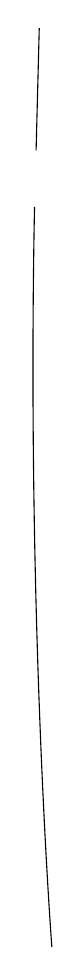
\begin{tikzpicture}[x=1cm,y=1cm]
\draw (0,0) -- (-0.04,-1.55);
\draw (-0.06,-2.27) .. controls (-0.14,-6.3) and (0.04,-10.0) .. (0.16,-11.67);
\end{tikzpicture}}}

We have a group $\Gamma$ of \unsure{automorphisms} of $\mathcal X$ ($\Gamma$ profinite in the profinite case --- to do things properly we should spell out the reasonable hypotheses to be made to take account of the profinite topology of $\Gamma$\ldots). We put
\[
\Pi=\Pi_1(\mathcal X,x_0),\quad \mathcal M=\Pi_1(\mathcal X,\Gamma;x_0)\qquad\text{hence}
\]
\inserted{\diagram{\begin{tikzcd}[column sep=large]
{(*)}\quad 1 \arrow[r,no head] & \Pi \arrow[r,no head] & \mathcal M \arrow[r,no head] & \Gamma \arrow[r] & 1
\end{tikzcd}}}
we give ourselves a quotient $M$ of $\Pi$, \deleted{\unsure{a}} by a normal subgroup \uline{in $\mathcal M$}, \unsure{or} what amounts to the same thing a quotient of $\Pi_{\mathrm{ab}}=\Pi/[\Pi,\Pi]$ stable under the action of $\Gamma$, \deleted{for}\inserted{hence} a \deleted{$\widetilde{\mathcal M}=\mathcal M/$} quotient extension of $(*)$,
\[
(287)\qquad
\diagram{\begin{tikzcd}[column sep=large]
1 \arrow[r] & M \arrow[r,no head] & \widetilde{\mathcal M} \arrow[r,no head] & \Gamma \arrow[r,no head] & 1
\end{tikzcd}}
\]
where $M$ is \unsure{commutative|commutative} so $\Gamma$ operates on $M$.

We are interested in the category of coverings \deleted{$\unsure{M_{\mathcal X}}$-torsors $\mathcal X'_0$ \unsure{over}} $\mathcal X'$ of $(\mathcal X,\Gamma)$, satisfying the conditions

\margin{129}

\begin{center}
\small
129\\
\texttt{https://grothendieck.umontpellier.fr}\\
Université de Montpellier, UMR CNRS 5149, Case courrier 051, Place Eugène Bataillon\\
34095 Montpellier cedex 5 - France
\end{center}

\scanpage{131}
\mspage{713}

Following : after forgetting the operations of $\Gamma$, we find a \inserted{connected} Galois covering \inserted{\unsure{(and even abelian)}} of $\mathcal X$, corresponding to the quotient group $M$ of $\Pi=\Pi_1(\mathcal X,x_0)$ --- so that $\mathcal X'$ becomes in a natural way a torsor under $M_{\mathcal X}$.
\margin{\figure{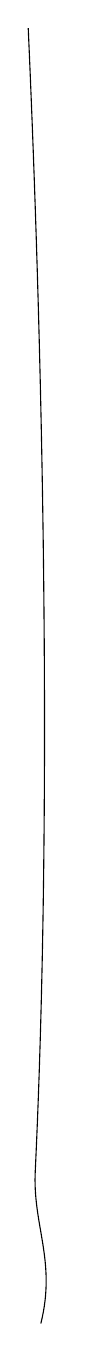
\begin{tikzpicture}[x=1cm,y=1cm]
\draw (0,0) .. controls (0.2,-4.5) and (0.3,-10.0) .. (0.09,-14.5) .. controls (0.05,-15.2) and (0.36,-15.65) .. (0.16,-16.45);
\end{tikzpicture}}}
The functor
\[
\mathcal X'\longmapsto\mathcal X'(x_0)\qquad\text{(fiber at $x_0$)}
\]
from the category of these $\mathcal X'$ to the category of sets, in fact goes to the sets $E$ equipped with the following structures

\noindent a) $E$ is an $M$-torsor, and as such gives rise to an extension
\diagram{\begin{tikzcd}[column sep=large]
1 \arrow[r,no head] & M \arrow[r] & \operatorname{Aff}(E) \arrow[r] & \operatorname{Aut}(M) \arrow[r,no head] & 1
\end{tikzcd}}
hence an \unsure{induced} subextension
\[
(288)\qquad
\diagram{\begin{tikzcd}[column sep=large]
1 \arrow[r,no head] & M \arrow[r,no head] & \operatorname{Aff}_{\Gamma}(E) \arrow[r] & \widetilde\Gamma \arrow[r,no head] & 1
\end{tikzcd}}
\]
where
\[
\widetilde\Gamma=\operatorname{Im}(\Gamma\longrightarrow\operatorname{Aut}(M)).
\]

\noindent b) We have a homomorphism of extensions
\[
(289)\qquad
\diagram{\begin{tikzcd}[column sep=large,row sep=large]
1 \arrow[r,no head] & M \arrow[r,no head] \arrow[d,Rightarrow,"\mathrm{id}"] & \widetilde{\mathcal M} \arrow[r,no head] \arrow[d,"\Theta_{\widetilde{\mathcal M}}"] & \Gamma \arrow[r,no head] \arrow[d,"\mathrm{can}"] & 1 \\
1 \arrow[r,no head] & M \arrow[r,no head] & \operatorname{Aff}_{\Gamma}(E) \arrow[r,no head] & \widetilde\Gamma \arrow[r,no head] & 1
\end{tikzcd}}\qquad .
\]
The category of the $\mathcal X'$ (with isomorphisms\ldots) is equivalent to that of \deleted{$\unsure{M}$} pairs $(E,\Theta_{\widetilde{\mathcal M}})$, where $E$ is an $M$-torsor, and $\Theta_{\widetilde{\mathcal M}}$ a homomorphism of extensions (289).

\margin{130}

\begin{center}
\small
130\\
\texttt{https://grothendieck.umontpellier.fr}\\
Université de Montpellier, UMR CNRS 5149, Case courrier 051, Place Eugène Bataillon\\
34095 Montpellier cedex 5 - France
\end{center}

\scanpage{132}

The automorphisms of an object $\mathcal X'$ correspond to ``translations'' by elements of $M^\Gamma$\inserted{$=\operatorname{Cent}(\widetilde{\mathcal M})$}, (\unsure{in} the terms of $E,\Theta_{\widetilde{\mathcal M}}$) to translations of $E$ by \deleted{such \unsure{elements|elements}} elements of $M^\Gamma$, \deleted{which in \unsure{so far}}\inserted{(in so far} as elements of $\operatorname{Aff}_{\Gamma}(E)$ they are central, and by conjugating by these elements we find the \uline{same} homomorphism $\Theta_{\widetilde{\mathcal M}}$\ldots).
\margin{\figure{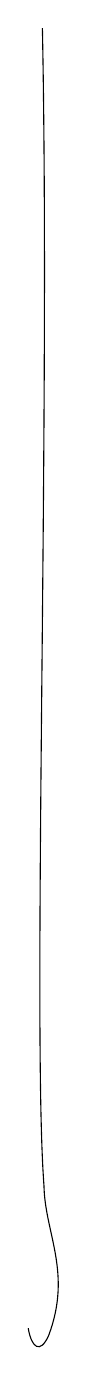
\begin{tikzpicture}[x=1cm,y=1cm]
\draw (0,0) .. controls (0.10,-5.0) and (-0.13,-12.7) .. (0.02,-14.7) .. controls (0.03,-15.3) and (0.38,-15.8) .. (0.08,-16.6) .. controls (-0.03,-16.85) and (-0.14,-16.75) .. (-0.18,-16.51);
\end{tikzpicture}}}
The isomorphism classes of such \unsure{elements} \deleted{\unsure{identify}}\inserted{\unsure{correspond}} one-to-one to the $M$-conjugacy classes of splittings of the extension (287) of $\Gamma$ by $\widetilde{\mathcal M}$. In precise terms, to an $(E,\Theta_{\widetilde{\mathcal M}})$ is associated \unsure{canonical|canonically} a \deleted{$\unsure{M}$} homomorphism of $M$-sets
\[
(290)\qquad
\diagram{\begin{tikzcd}[column sep=large]
E \arrow[r] & \operatorname{Scind}(\widetilde{\mathcal M}\ \unsure{\text{extension}}\ \text{of }\Gamma\ \text{by }M)
\end{tikzcd}}
\]
whose image is the conjugacy class \unsure{describing} the isomorphism class under consideration. \deleted{\unsure{The image}}\inserted{The homomorphism} (290) \unsure{is|of} factored through $M^\Gamma\backslash E$ as a \uline{monomorphism}
\[
(291)\qquad
\diagram{\begin{tikzcd}[column sep=large]
M^\Gamma\backslash E \arrow[r,hook] & \operatorname{Scind}(\widetilde{\mathcal M}\ \text{extension of }\Gamma\ \text{by }M)
\end{tikzcd}},
\]
and if $M^\Gamma=0$, we see that $E$ is canonically reconstructed from the class of

\margin{131}

\begin{center}
\small
131\\
\texttt{https://grothendieck.umontpellier.fr}\\
Université de Montpellier, UMR CNRS 5149, Case courrier 051, Place Eugène Bataillon\\
34095 Montpellier cedex 5 - France
\end{center}

\scanpage{133}
\mspage{714}

conjugacy under consideration. The \inserted{(affine)} operation of $\widetilde{\mathcal M}$ on $E$ \inserted{(defined by $\Theta_{\widetilde{\mathcal M}}$)} is none other than the operation \deleted{of} \inserted{(\unsure{induced} by the)} conjugation on \inserted{the set} of splittings (which of course does not take one out of an $M$-conjugacy class, even when conjugating by arbitrary elements of $\widetilde{\mathcal M}$).
\margin{\figure{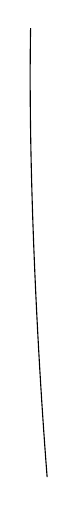
\begin{tikzpicture}[x=1cm,y=1cm]
\draw (0,0) .. controls (-0.03,-1.65) and (0.07,-3.9) .. (0.21,-5.7);
\end{tikzpicture}}}

\uline{Corollary} Suppose we have
\[
(292)\qquad \underbrace{H^0(\widetilde\Gamma,M)}_{M^\Gamma}=H^1(\widetilde\Gamma,M)=0
\]
i.e. that \deleted{\unsure{all|all}} two splittings of a trivial extension of $\widetilde\Gamma$ by $M$ are conjugate by a unique element of $M$. This implies \inserted{therefore (because of $M^\Gamma=\unsure{\{0\}|0}$)} that the category of the $\mathcal X'$, or again that of the pairs $(E,\Theta_{\widetilde{\mathcal M}})$, is rigid, \deleted{Then the classes} \inserted{i.e. an object is known up to an isomorphism} which is unique when we know its isomorphism class. This being so, the isomorphism classes in question \deleted{correspond}\inserted{(i.e. the classes} of \deleted{$M$-\unsure{conjugation|conjugation}} conjugacy of the splittings of \deleted{one-to-one} the extension $\widetilde{\mathcal M}$ of $\Gamma$ by $M$) correspond one-to-one to the quotient groups $\widetilde{\widetilde{\mathcal M}}$
\margin{\figure{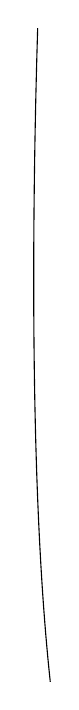
\begin{tikzpicture}[x=1cm,y=1cm]
\draw (0,0) .. controls (-0.06,-1.95) and (-0.12,-5.7) .. (0.16,-8.3);
\end{tikzpicture}}}

\margin{132}

\begin{center}
\small
132\\
\texttt{https://grothendieck.umontpellier.fr}\\
Université de Montpellier, UMR CNRS 5149, Case courrier 051, Place Eugène Bataillon\\
34095 Montpellier cedex 5 - France
\end{center}
